Software engineering requires rigorous testing of rapidly evolving programs,
which costs manpower comparable to developing the product itself.  To guarantee
programs' compliance with the specification, we need testers that can tell
compliant implementations from violating ones.

This thesis studies the testing of interactive systems' semantics: The system
under test (SUT) interacts with the tester by sending and receiving messages,
and the tester determines whether the messages sent by the SUT are valid or not
with respect to the protocol specification.

This section introduces the basic concepts of interactive testing
(\autoref{sec:interactive-testing}), why nondeterminism made this problem
difficult
(Sections~\ref{sec:internal-external-nondeterminism}--\ref{sec:inter-execution-nondeterminism}),
and how language designs address the challenges introduced by nondeterminism
(\autoref{sec:contribution}).

\section{Interactive Testing}
\label{sec:interactive-testing}
Suppose we want to test a web server that supports GET and PUT methods:
\begin{lstlisting}[style=customcoq]
  CoFixpoint server (data: key -> value) :=
    request <- recv;;
    match request with
    | GET k   => send (data k);; server  data
    | PUT k v => send  Done   ;; server (data [k |-> v])
    end.
\end{lstlisting}
We can write a tester client that interacts with the server and determines
whether it behaves correctly:
\begin{lstlisting}[style=customcoq]
  CoFixpoint tester (data: key -> value) :=
    request <- random;;
    send request;;
    response <- recv;;
    match request with
    | GET k   => if response =? data k
                 then tester data
                 else reject
    | PUT k v => if response =? Done
                 then tester (data [k |-> v])
                 else reject
    end.
\end{lstlisting}
This tester implements a reference server internally that computes the expected
behavior.  The behavior is then compared against that produced by the SUT.  The
tester rejects the SUT upon any difference from the computed expectation.

The above tester can be viewed as two modules: (i) a {\em test harness} that
interacts with the server and produces transactions of sends and receives, and
(ii) a {\em validator} that determines whether the transactions are valid or
not:
\begin{lstlisting}[style=customcoq]
  (* Compute the expected response and next state of the server. *)
  Definition serverSpec request data :=
    match request with
    | GET k   => (data k, data)
    | PUT k v => (Done  , data [k |-> v])
    end.
  (* Validate the transaction against the stateful specification. *)
  Definition validate spec request response data :=
    let (expect, next) := spec request data in
    if response =? expect then Success next else Failure.
  (* Produce transactions for the validator. *)
  CoFixpoint harness validator state :=
    request <- random;;
    send request;;
    response <- recv;;
    if validator request response state is Success next
    then harness validator next
    else reject.
  Definition tester := harness (validate serverSpec).
\end{lstlisting}
Such testing method works for deterministic systems, whose behavior can be
precisely computed from its input.  Whereas, many systems are allowed to behave
nondeterministically.  How to test systems that involve randomness?  How to
validate servers' behavior against concurrent clients?  The following sections
discuss nondeterminism by partitioning it in two ways, and explains how they
pose challenges to the validator and the test harness.

\section{Internal and external nondeterminism}
\label{sec:internal-external-nondeterminism}
When people talk to each other, voice is transmitted over substances.  When
testers interact with the SUT, messages are transmitted via the runtime
environment.  The specification might allow SUTs to behave differently from each
other, just like people speaking in different accents, we call it {\em internal
  nondeterminism}.  The runtime environment might affect the transmission of
messages, just like solids transmit voice faster than liquids and gases, we call
it {\em external nondeterminism}.

\subsection{Internal nondeterminism}
Within the SUT, correct behavior may be \mbox{underspecified}.  For example,
HTTP~\cite{rfc7232} allows requests to be conditional: If the client has a local
copy of some resource and the copy on the server has not changed, then the
server needn't resend the resource.  To achieve this, an HTTP server may
generate a short string, called an ``entity tag'' (ETag), identifying the
content of some resource, and send it to the client:
\begin{center}
  \begin{minipage}[t]{.4\textwidth}
    \begin{lstlisting}[style=customc]
/* Client: */
GET /target HTTP/1.1
    \end{lstlisting}
  \end{minipage}\begin{minipage}[t]{.4\textwidth}
    \begin{lstlisting}[style=customc]
/* Server: */
HTTP/1.1 200 OK
ETag: "tag-foo"
... content of /target ...
    \end{lstlisting}
  \end{minipage}
\end{center}
The next time the client requests the same resource, it can include the ETag in
the GET request, informing the server not to send the content if its ETag still
matches:
\begin{center}
\begin{minipage}[t]{.4\textwidth}
\begin{lstlisting}[style=customc]
/* Client: */
GET /target HTTP/1.1
If-None-Match: "tag-foo"
\end{lstlisting}
\end{minipage}\begin{minipage}[t]{.4\textwidth}
\begin{lstlisting}[style=customc]
/* Server: */
HTTP/1.1 304 Not Modified
\end{lstlisting}
\end{minipage}
\end{center}
If the ETag does not match, the server responds with code 200 and the updated
content as usual.

Similarly, if a client wants to modify the server's resource atomically by
compare-and-swap, it can include the ETag in the PUT request as
\inlinec{If-Match} precondition, which instructs the server to only update the
content if its current ETag matches:
\begin{center}
  \begin{minipage}[t]{.4\textwidth}
    \begin{lstlisting}[style=customc]
/* Client: */
PUT /target HTTP/1.1
If-Match: "tag-foo"
... content (A) ...
    \end{lstlisting}
  \end{minipage}
  \begin{minipage}[t]{.4\textwidth}
    \begin{lstlisting}[style=customc]
/* Server: */
HTTP/1.1 204 No Content
    \end{lstlisting}
  \end{minipage}

  \begin{minipage}[t]{.4\textwidth}
    \begin{lstlisting}[style=customc]
/* Client: */
GET /target HTTP/1.1
    \end{lstlisting}
  \end{minipage}
  \begin{minipage}[t]{.4\textwidth}
    \begin{lstlisting}[style=customc]
/* Server: */
HTTP/1.1 200 OK
ETag: "tag-bar"
... content (A) ...
    \end{lstlisting}
  \end{minipage}
\end{center}
If the ETag does not match, then the server should not perform the requested
operation, and should reject with code 412:
\begin{center}
  \begin{minipage}[t]{.4\textwidth}
    \begin{lstlisting}[style=customc]
/* Client: */
PUT /target HTTP/1.1
If-Match: "tag-baz"
... content (B) ...
    \end{lstlisting}
  \end{minipage}
  \begin{minipage}[t]{.4\textwidth}
    \begin{lstlisting}[style=customc]
/* Server: */
HTTP/1.1 412 Precondition Failed
    \end{lstlisting}
  \end{minipage}

  \begin{minipage}[t]{.4\textwidth}
    \begin{lstlisting}[style=customc]
/* Client: */
GET /target HTTP/1.1
    \end{lstlisting}
  \end{minipage}
  \begin{minipage}[t]{.4\textwidth}
    \begin{lstlisting}[style=customc]
/* Server: */
HTTP/1.1 200 ok
ETag: "tag-bar"
... content (A) ...
    \end{lstlisting}
  \end{minipage}
\end{center}
Whether a server's response should be judged {\em valid} or not depends on the
ETag it generated when creating the resource.  If the tester doesn't know the
server's internal state ({\it e.g.}, before receiving any 200 response that
includes an ETag), and cannot enumerate all of them (as ETags can be arbitrary
strings), then it needs to maintain a space of all possible values, and narrow
the space upon further interactions with the server.  For example, ``If the
server has revealed some resource's ETag as \inlinec{"tag-foo"}, then it must
not reject requests targetting this resource conditioned over \inlinec{If-Match:
  "tag-foo"}, until the resource has been modified''; and ``Had the server
previously rejected an \inlinec{If-Match} request, it must reject the same
request until its target has been modified.''

\begin{figure}
\begin{lstlisting}[style=customcoq]
  Definition validate request response
             (data      : key -> value)
             (tag_is    : key -> Maybe etag)
             (tag_is_not: key -> list etag) :=
    match request, response with
    | PUT k t v, NoContent => 
      if t \in tag_is_not k then Failure
      else if (tag_is k =? Unknown) || strong_match (tag_is k) t
      then (* Now the tester knows that the data in [k]
            * is updated to [v], but its new ETag is unknown. *)
        Success (data       [k |-> v],
                 tag_is     [k |-> Unknown],
                 tag_is_not [k |-> [] ])
      else Failure
    | PUT k t v, PreconditionFailed =>
      if strong_match (tag_is k) t then Failure
      else (* Now the tester knows that the ETag of [k]
            * is other than [t]. *)
        Success (data, tag_is, tag_is_not [k |-> t::(tag_is_not k)])
    | GET k t, NotModified =>
      if t \in tag_is_not then Failure
      else if (tag_is k =? Unknown) || weak_match (tag_is k) t
      then (* Now the tester knows that the ETag of [k]
            * is equal to [t]. *)
        Success (data, tag_is [k |-> Known t], tag_is_not)
      else Failure
    | GET k t0, OK t v =>
      if weak_match (tag_is k) t0 then Failure
      else if data k =? v
      then (* Now the tester knows the ETag of [k]. *)
        Success (data, tag_is [k |-> Known t], tag_is_not)
      else Failure
    | _, _ => Failure
    end.
\end{lstlisting}
  \caption[Ad hoc tester for \http conditional requests.]{Ad hoc tester for
    \http conditional requests.  \ilc{PUT k t v} represents a PUT request that
    changes \ilc k's value into \ilc v only if its ETag matches \ilc t; \ilc{GET
      k t} is a GET request for \ilc k's value only if its ETag does not match
    \ilc t; \ilc{OK t v} indicates that the request target's value is \ilc v and
    its ETag is \ilc t.}
  \label{fig:etag-tester}
\end{figure}

This idea of remembering matched and mismatched ETags is implemented in
\autoref{fig:etag-tester}.  For each key, the validator maintains three internal
states: (i) The value stored in \ilc{data}, (ii) the corresponding resource's
ETag, if known by the tester, stored in \ilc{tag_is}, and (iii) ETags that
should not match with the resource's, stored in \ilc{tag_is_not}.  Each pair of
request and response contributes to the validator's knowledge of the target
resource.  The tester rejects the SUT if the observed behavior does not match
its knowledge gained in previous interactions.

Even a simple nondeterminism like ETags requires such careful design of the
validator, based on thorough comprehension of the specification.  For more
complex protocols, we hope to construct the validator in a reasonable way.

\subsection{External nondeterminism}
To discuss the nondeterminism caused by the environment, we need to define the
environment concept in testing scenario.
\begin{definition}[Environment, input, output, and observations]
  {\em Environment} is the substance that the tester and the SUT interact with.
  {\em Input} is the subset of the environment that the tester can manipulate.
  {\em Output} is the subset of the environment that the SUT can alter.  {\em
    Observation} is the tester's view of the environment.
\end{definition}
When testing servers, the environment is the network stack between the client
and the server.  The input is the request sent by the client, and the output is
the response sent by the server.  The response is transmitted via the network,
until reaching the client side as observations.

\begin{figure}
  \centering
  \begin{minipage}[c]{.3\textwidth}
\begin{lstlisting}[style=customcoq]
  (* Observation: *)
  1> PUT k "new"
  1< Done
  2> GET k
  2< "new"
\end{lstlisting}
  \end{minipage}\begin{minipage}[c]{.4\textwidth}
  \includegraphics[width=\linewidth]{figures/linear-trace}
  \end{minipage}\begin{minipage}[c]{.3\textwidth}
\begin{lstlisting}[style=customcoq]
  (* Output: *)
  1> PUT k "new"
  1< Done
  2> GET k
  2< "new"
\end{lstlisting}
  \end{minipage}
  \caption[Linear trace upon no concurrency.]{Upon no concurrency, the
    observation is identical to the output.}
  \label{fig:linear-trace}
\end{figure}
\begin{figure}
  \centering
  \begin{minipage}[c]{.3\textwidth}
\begin{lstlisting}[style=customcoq]
  (* Observation: *)
  1> PUT k "new"
  2> GET k
  1< Done
  2< "old"
\end{lstlisting}
  \end{minipage}\begin{minipage}[c]{.4\textwidth}
    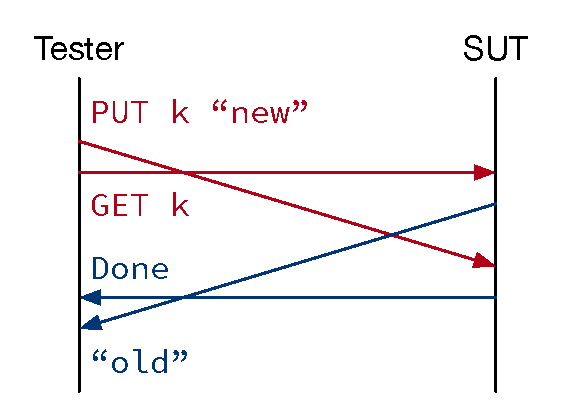
\includegraphics[width=\linewidth]{figures/network-trace}
  \end{minipage}\begin{minipage}[c]{.3\textwidth}
\begin{lstlisting}[style=customcoq]
  (* Output: *)
  2> GET k
  2< "old"
  1> PUT k "new"
  1< Done
\end{lstlisting}
  \end{minipage}
  \caption[Reordered trace upon network delays.]{Acceptable: The observation can
    be explained by a valid output reordered by the network environment.}
  \label{fig:reordered-trace}
\end{figure}
\begin{figure}
  \centering
  \begin{minipage}[c]{.3\textwidth}
\begin{lstlisting}[style=customcoq]
  (* Observation: *)
  1> PUT k "new"
  1< Done
  2> GET k
  2< "old"
\end{lstlisting}
  \end{minipage}\begin{minipage}[c]{.4\textwidth}
  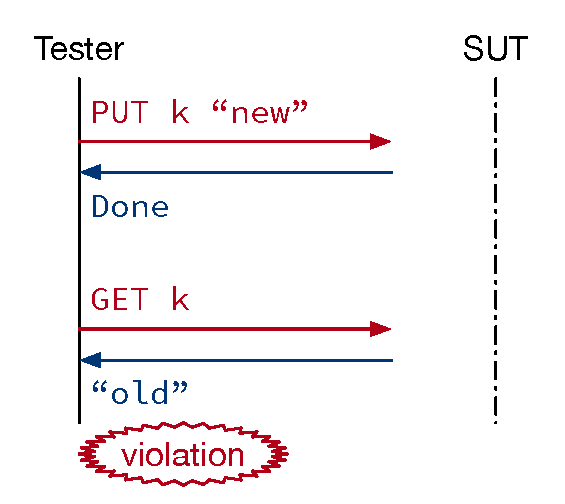
\includegraphics[width=\linewidth]{figures/invalid-trace}
  \end{minipage}\begin{minipage}[c]{.3\textwidth}\
  \end{minipage}
  \caption[Invalid trace that violates the specification.]{Unacceptable: The
    tester received the \ilc{Done} response before sending the \ilc{GET}
    request, thus the SUT must have processed the \ilc{PUT} request before the
    \ilc{GET} request.  Therefore, the \ilc{"old"} response must be invalid.}
  \label{fig:invalid-trace}
\end{figure}
The tester shown in \autoref{sec:interactive-testing} runs one client at a time.
It waits for the response before sending the next request, as shown in
\autoref{fig:linear-trace}.  Such tester's observation is guaranteed identical
to the SUT's output, so it only needs to scan the requests and responses with
one stateful validator.

To reveal the server's behavior upon concurrent requests, the tester needs to
simulate multiple clients, sending new requests before receiving previous
responses.  The network delay might cause the server to receive requests in a
different order from that on the tester side.  Vice versa, responses sent by the
server might be reordered before arriving at the tester, as shown in
\autoref{fig:reordered-trace}.  Such tester's observation can be explained by
various outputs on the SUT side.  The validator needs to consider all possible
outputs that can explain such observation, and see if anyone of them complies
with the specification.  If no valid output can explain the observation, then
the tester should reject the SUT, as shown in \autoref{fig:invalid-trace}.

We hope to construct a tester that can handle external nondeterminism
systematically, and provide a generic way for reasoning on the environment.

\section{Test harness and inter-execution nondeterminism}
\label{sec:inter-execution-nondeterminism}
A good tester consists of (i) a validator that accurately determines whether its
observations are valid or not, and (ii) a test harness that can reveal invalid
observations effectively.  \autoref{sec:internal-external-nondeterminism} has
explained the challenges in the validator.  Here we discuss the test harness.

\subsection{Test harness}

\begin{figure}
  Validator, generator, shrinker
  \caption{Tester architecture.}
  \label{fig:test-harness}
\end{figure}
Explain \autoref{fig:test-harness}.

\subsection{Inter-execution nondeterminism}
\begin{figure}
  Server example, preferably using timestamps.
  \caption{Inter-execution nondeterminism}
  \label{fig:inter-execution}
\end{figure}
Explain \autoref{fig:inter-execution}.

\lys{Inter-execution nondeterminism is usually mentioned in parallel with
  inter-implementation nondeterminism, but the latter concept doesn't contribute
  to this thesis, thus ignoring.}


\section{Contribution}
\label{sec:contribution}
\lys{To be polished.}
To address the challenges in testing caused by different forms of
nondeterminism, I introduce symbolic languages for writing specifications and
representing test cases:

\begin{enumerate}
\item The specification is written as a reference implementation---a
nondeterministic program that exhibits all possible behavior allowed by
the protocol.  Inter-implementation and inter-execution uncertainties are
represented by symbolic variables, and the space of nondeterministic behavior is
defined by all possible assignments of the variables.

The validator is derived from the reference implementation, by {\em
  dualising} the server-side program into a client-side observer.

\item Test generation heuristics are defined as computations from the observed
trace (list of sent and received messages) to the next message to send.  I
introduce a symbolic intermediate representation for specifying the relation
between the next message and previous messages.

\item The symbolic language for generating test cases also enables effective
shrinking of test cases.  The test harness minimizes the counterexample by
shrinking its symbolic representation.  When running the test with a shrunk
input, the symbolic representations can be re-instantiated into request messages
that reflect the original heuristics.
\end{enumerate}

\subsection*{Thesis claim}
Symbolic abstract representation can address challenges in testing networked
systems with uncertain behavior.  Specifying protocols with symbolic reference
implementation enables validating the system's behavior systematically.
Representing test input as abstract messages allows generating and shrinking
interesting test cases.  Combining these methods result in a rigorous tester
that can capture protocol violations effectively.

This claim is supported by the following publications:
\begin{enumerate}
\item {\it From C to Interaction Trees: Specifying, Verifying, and Testing a
  Networked Server}~\cite{cpp19}, with Nicolas Koh, Yao Li, Li-yao Xia, Lennart
  Beringer, Wolf Honor\'e, and William Mansky, where I developed a tester
  program based on the swap server's ITree specification, and evaluated the
  tester's effectiveness by mutation testing.
\item {\it Verifying an HTTP Key-Value Server with Interaction Trees and
  VST}~\cite{itp21}, with Hengchu Zhang, Wolf Honor\'e, Nicolas Koh, Yao Li,
  Li-yao Xia, Lennart Beringer, and William Mansky, where I developed the
  top-level specification for \http, and derived a tester client that revealed
  liveness and interrupt-handling bugs in our HTTP server, despite it was
  formally verified.
\item {\it Model-Based Testing of Networked Applications}~\cite{issta21}, which
  describes my technique of specifying \http with symbolic reference
  implementations, and from the specification, automatically deriving a tester
  program that can find bugs in Apache and Nginx.
\item {\it Testing by Dualization} (to be submitted to OOPSLA), a theory for
  interactive testing, explaining how to specify protocols using abstract model
  implementations, and how to guarantee the soundness and completeness of the
  validator logic derived from the abstract model.
\end{enumerate}

This thesis is structured as follows:
